\section{misura di Peano-Jordan}

In questo capitolo vogliamo dare una definizione di \emph{misura} di un
sottoinsieme $E\subset \RR^n$ formalizzando le stesse nozioni che sostanzialmente
venivano già usate dagli antichi greci.
Lo faremo nel caso per noi più rilevante ovvero il caso planare $n=2$ in cui la \emph{misura}
di un insieme si chiama \emph{area}.
Ma l'intera costruzione potrebbe essere fatta senza
nessuna difficoltà (se non per le notazioni che si complicano) nel caso generale della
dimensione $n$.

Dato un insieme $E\subset \RR^2$ vorremmo definire la sua area $m(E)\in \RR$
in modo che valgano le seguenti proprietà:
\begin{enumerate}
  \item se $E\cap F=\emptyset$ allora $m(E\cup F) = m(E) + m(F)$ (additività);
  \item se $E \subset F$ allora $m(E) \le m(F)$ (monotonia);
  \item se $E=[x_1,x_2]\times [y_1,y_2]$
  allora $m(E) = \abs {x_2-x_1}\cdot \abs{y_2-y_1}$ (normalizzazione).
\end{enumerate}

Andremo a definire la misura $m$ su una famiglia di sottoinsiemi di $\RR^2$ che
chiameremo \emph{misurabili} secondo Peano-Jordan.
Si potrebbe dimostrare che non è possibile definire $m$ su tutti i sottoinsiemi di $\RR^2$
in modo che valgano le proprietà enunciate qui sopra.
Sarebbe però possibile
definire la misura su una classe molto più amplia di insiemi di quelli che andremo a considerare noi, 
imponendo l'additività non solo su unioni finite ma anche su unioni numerabili
($\sigma$ additività).
Quello che si otterrebbe
è la cosiddetta misura di \emph{Lebesgue} che è ormai una costruzione standard
dell'analisi matematica ma richiederebbe una teoria molto più complessa da sviluppare.
Ci accontenteremo qui di introdurre la misura $m$ (misura finitamente additiva) 
di Peano-Jordan
che poi ci permetterà di dare significato geometrico all'integrale di Riemann.
\index{misura!di Peano-Jordan}%
\index{Peano-Jordan!misura di}%
\index{additiva!misura}%

Diremo che un insieme $R\subset \RR^2$ è un
\emph{rettangolo cartesiano}%
\mymargin{rettangolo cartesiano}%
\index{rettangolo!cartesiano}
se $R$ è il prodotto cartesiano di due intervalli limitati
cioè
\[
  R = I\times J
\]
con $x_1=\inf I>-\infty$,
$x_2=\sup I<+\infty$,
$y_1=\inf J > -\infty$,
$y_2=\sup J < +\infty$.

Se $I=[x_1,x_2]$ e $J=[y_1,y_2]$ allora,
affinché valga la proprietà di normalizzazione,
dovremo porre:
\[
  m([x_1,x_2]\times[y_1,y_2]) = \abs{x_2-x_1}\cdot\abs{y_2-y_1}.
\]

Se $I=(x_1,x_2)$ e $J=(y_1,y_2)$ sono intervalli aperti (e limitati) allora
per ogni $\eps>0$ con $\eps<(x_2-x_1)/2$ e $\eps<(y_2-y_1)/2$ si ha
\[
  [x_1+\eps,x_2-\eps] \times [y_1+\eps,y_2-\eps]
  \subset (x_1,x_2)\times (y_1,y_2)
  \subset [x_1,x_2]\times [y_1,y_2]
\]
da cui, affinché valga la proprietà di monotonia, si dovrà avere:
\[
  (x_2-x_1-2\eps)\cdot (y_2-y_1-2\eps) \le m((x_1,x_2)\times(y_1,y_2)) \le \abs{x_2-x_1}\cdot \abs{y_2-y_1}.
\]
Ma affinché questo sia vero per ogni $\eps>0$ si dovrà necessariamente
porre:
\[
  m((x_1,x_2)\times(y_1,y_2)) = \abs{x_2-x_1}\cdot\abs{y_2-y_1}.
\]
Lo stesso vale se gli intervalli sono semiaperti o comunque
se consideriamo qualunque insieme $E$ tale che $(x_1,x_2)\times (y_1,y_2) \subset E \subset [x_1,x_2]\times[y_1,y_2]$.
Dunque l'area di un rettangolo non cambia se aggiungiamo o togliamo punti
dai suoi lati.

Se un insieme $E\subset \RR^2$ può essere scritto come unione finita
di rettangoli disgiunti:
\[
  E = R_1 \cup R_2 \cup \dots \cup R_N
  \qquad
  R_i \cap R_j=\emptyset\text{ se } i\neq j
\]
diremo che $E$ è un \emph{polirettangolo cartesiano}%
\mymargin{polirettangolo cartesiano}%
\index{polirettangolo!cartesiano}.
In tal caso per garantire l'additività dell'area
porremo:
\[
  m(E) = m(R_1) + \dots + m(R_N).
\]
Affinché questa sia una buona definizione dobbiamo verificare che
se $A$ può essere scritto come unione di rettangoli disgiunti in due modi
diversi, allora la somma delle misure dei rettangoli dà lo stesso
risultato con entrambe le decomposizioni.
Questo è intuitivamente ovvio, e dipende dal fatto che date due
diverse decomposizioni in rettangoli è possibile considerare
una griglia formata da tutte le rette che contengono i lati di ogni rettangolo.
Questa griglia identifica una decomposizione in rettangolini che possono essere
utilizzati per ricostruire sia l'una che l'altra decomposizione.
Ogni rettangolo delle due decomposizioni sarà unione di rettangolini e la sua
area sarà la somma delle aree dei rettangolini. Ma visto che le due
decomposizioni si suddividono negli stessi rettangolini, le aree definite
dalle due decomposizioni devono coincidere.

\begin{figure}
  \hfill
  \subcaptionbox{}
  {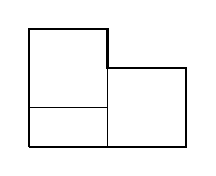
\begin{tikzpicture}[x=0.5cm, y=0.5cm]
      \draw[thick] (1,1) -- (5,1) -- (5,3) -- (3,3) -- (3,4) -- (1,4) -- (1,1);
      \draw (1,2) -- (3,2);
      \draw (3,1) -- (3,3);
  \end{tikzpicture}}
  \hfill
  \subcaptionbox{}
  {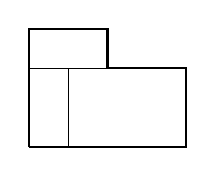
\begin{tikzpicture}[x=0.5cm, y=0.5cm]
      \draw[thick] (1,1) -- (5,1) -- (5,3) -- (3,3) -- (3,4) -- (1,4) -- (1,1);
      \draw (1,3) -- (3,3);
      \draw (2,1) -- (2,3);
  \end{tikzpicture}}
  \hfill
  \subcaptionbox{}
  {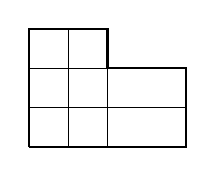
\begin{tikzpicture}[x=0.5cm, y=0.5cm]
      \draw[thick] (1,1) -- (5,1) -- (5,3) -- (3,3) -- (3,4) -- (1,4) -- (1,1);
      \draw (1,2) -- (5,2);
      \draw (1,3) -- (3,3);
      \draw (2,1) -- (2,4);
      \draw (3,1) -- (3,4);
  \end{tikzpicture}}
  \hfill\mbox{}
  \caption{Lo stesso polirettangolo si può ottenere
  come due diverse unioni di rettangoli: (a), (b). Prendendo in considerazione
  tutte le rette che contengono i lati di tutti i rettangoli coinvolti si
  ottiene una suddivisione (c) per cui ogni rettangolo in (a) o in (b) è unione di rettangoli in (c).}
\end{figure}

Per lo stesso motivo risulta chiaro che se $E$ e $F$ sono due polirettangoli
anche $E\cup F$, $E \cap F$, $E\setminus F$  e $F\setminus E$ sono polirettangoli e risulta
\begin{equation}\label{eq:48474624}
  m(E \cup F) = m(E\setminus F) + m(E\cap F) + m(F\setminus E).
\end{equation}
Infatti è possibile trovare una famiglia di rettangolini (quelli identificati
dalla griglia di tutte le rette contenenti i lati dei rettangoli di $E$ e dei rettangoli di $F$)
che sono tra loro disgiunti e tali che
$E\cap F$, $E\setminus F$ e $F\setminus E$
possono essere scritti come unione di questi rettangolini. Questi insiemi
sono tra loro disgiunti e quindi, scrivendo l'area di ognuno come la somma delle
aree dei rettangoli, si trova~\eqref{eq:48474624}.

Se ora prendiamo un insieme $E\subset \RR^2$ qualunque
e imponiamo che valga la proprietà di monotonia,
dovremo avere che $m(E)$, se è definibile, deve
essere l'elemento di separazione tra le misure
dei polirettangoli contenuti in $E$ e di quelli contenenti $E$.
Si giustifica quindi la seguente.

\begin{definition}[misura di Peano-Jordan]
\label{def:peano-jordan}%
\mymargin{Peano-Jordan}%
\index{Peano-Jordan}%
\index{misura!di Peano-Jordan}%
\index{Peano-Jordan!misura di}%
\index{Jordan!misura di}%
Sia $E\subset \RR^2$ un insieme limitato. Definiamo:
\begin{align*}
m^*(E) &= \inf\ENCLOSE{m(F)\colon \text{$F\supset E$, $F$ polirettangolo}}, \\
m_*(E) &= \sup\ENCLOSE{m(F)\colon \text{$F\subset E$, $F$ polirettangolo}}.
\end{align*}

Visto che $E$ è limitato (dunque è contenuto in un rettangolo limitato)
si ha $m^*(E)<+\infty$ e visto che $\emptyset \subset E$
e $m(\emptyset)=0$ (l'insieme vuoto $\emptyset = (a,a) \times (c,c)$ è un
polirettangolo di area nulla) si ha $m_*(E)\ge 0$. Inoltre $m_*(E)\le m^*(E)$
in quanto ogni polirettangolo contenuto in $E$ è contenuto, e quindi ha area non superiore, 
ad ogni polirettangolo contenente $E$.

Se $m^*(E) = m_*(E)$ diciamo che $E$ è \emph{misurabile}%
\mymargin{misurabile}%
\index{misurabile} secondo Peano-Jordan
e poniamo $m(E) = m^*(E) = m_*(E)$ la sua misura di Peano-Jordan.
\end{definition}

\begin{theorem}[proprietà della misura di Peano-Jordan]
Se $E$ e $F$ sono Peano-Jordan misurabili allora anche
$E\cup F$, $E\setminus F$, $F\setminus E$, $E\cap F$
sono Peano-Jordan misurabili e risulta
\begin{align*}
  m(E\cup F)
  &= m(E\setminus F) + m(E\cap F) + m(F\setminus E)\\
  &= m(E) + m(F) - m(E\cap F).
\end{align*}
\end{theorem}
%
\begin{proof}
Osserviamo che un insieme $E$ è misurabile se e solo se
per ogni $\eps>0$ esistono dei polirettangoli $E_*, E^*$
con $E_* \subset E \subset E^*$ tali che $m(E^*)-m(E_*)<\eps$
(basta utilizzare la caratterizzazione di estremo superiore e inferiore).

\begin{figure}
  \centering\ifdefined\figurePJA

\begin{tikzpicture}[x=0.5cm, y=0.5cm]
  \draw[draw=none,fill=white] (0,0) -- (14,00) -- (14,10) -- (0,10) -- (0,0);
\draw[fill=black,draw=none] plot [smooth cycle] coordinates {(1,4) (5,3) (7,1) (9,5) (5,8) (1,6)};
\end{tikzpicture}
\else
\ifdefined\figurePJB
%% draw set B

\begin{tikzpicture}[x=0.5cm, y=0.5cm]
\draw[draw=none,fill=white] (0,0) -- (14,00) -- (14,10) -- (0,10) -- (0,0);
\draw[fill=black,draw=none] plot [smooth cycle] coordinates {(10,1) (13,4) (10,8) (6,4)};
\end{tikzpicture}
\else
%
\begin{tikzpicture}[x=0.5cm, y=0.5cm]
  % False
% 255 255 255
\draw[draw=red] 
(4.05,7.94)--(3.85,7.94)--(3.65,7.94)--(3.65,7.77)--(3.45,7.77)--(3.24,7.77)--(3.24,7.6)--(3.04,7.6)--(2.84,7.6)--(2.84,7.43)--(2.64,7.43)--(2.64,7.26)--(2.43,7.26)--(2.23,7.26)--(2.23,7.09)--(2.03,7.09)--(2.03,6.93)--(1.82,6.93)--(1.82,6.76)--(1.62,6.76)--(1.62,6.59)--(1.42,6.59)--(1.22,6.59)--(1.22,6.42)--(1.01,6.42)--(1.01,6.25)--(0.811,6.25)--(0.811,6.08)--(0.811,5.91)--(0.608,5.91)--(0.608,5.74)--(0.608,5.57)--(0.405,5.57)--(0.405,5.41)--(0.405,5.24)--(0.405,5.07)--(0.405,4.9)--(0.405,4.73)--(0.405,4.56)--(0.405,4.39)--(0.608,4.39)--(0.608,4.22)--(0.608,4.05)--(0.811,4.05)--(0.811,3.89)--(1.01,3.89)--(1.01,3.72)--(1.22,3.72)--(1.42,3.72)--(1.62,3.72)--(1.62,3.55)--(1.82,3.55)--(2.03,3.55)--(2.23,3.55)--(2.43,3.55)--(2.43,3.38)--(2.64,3.38)--(2.84,3.38)--(3.04,3.38)--(3.24,3.38)--(3.24,3.21)--(3.45,3.21)--(3.65,3.21)--(3.85,3.21)--(4.05,3.21)--(4.26,3.21)--(4.26,3.04)--(4.46,3.04)--(4.66,3.04)--(4.66,2.87)--(4.86,2.87)--(5.07,2.87)--(5.07,2.7)--(5.27,2.7)--(5.27,2.53)--(5.47,2.53)--(5.47,2.36)--(5.47,2.2)--(5.68,2.2)--(5.68,2.03)--(5.68,1.86)--(5.88,1.86)--(5.88,1.69)--(5.88,1.52)--(6.08,1.52)--(6.08,1.35)--(6.28,1.35)--(6.28,1.18)--(6.28,1.01)--(6.49,1.01)--(6.49,0.845)--(6.69,0.845)--(6.89,0.845)--(7.09,0.845)--(7.09,1.01)--(7.3,1.01)--(7.3,1.18)--(7.5,1.18)--(7.5,1.35)--(7.7,1.35)--(7.7,1.52)--(7.7,1.69)--(7.91,1.69)--(7.91,1.86)--(8.11,1.86)--(8.11,2.03)--(8.11,2.2)--(8.31,2.2)--(8.31,2.36)--(8.31,2.53)--(8.51,2.53)--(8.51,2.7)--(8.51,2.87)--(8.51,3.04)--(8.72,3.04)--(8.72,3.21)--(8.72,3.38)--(8.92,3.38)--(8.92,3.55)--(8.92,3.72)--(8.92,3.89)--(8.92,4.05)--(9.12,4.05)--(9.12,4.22)--(9.12,4.39)--(9.12,4.56)--(9.12,4.73)--(9.12,4.9)--(9.12,5.07)--(9.12,5.24)--(9.12,5.41)--(8.92,5.41)--(8.92,5.57)--(8.72,5.57)--(8.72,5.74)--(8.72,5.91)--(8.51,5.91)--(8.51,6.08)--(8.31,6.08)--(8.31,6.25)--(8.11,6.25)--(8.11,6.42)--(7.91,6.42)--(7.91,6.59)--(7.7,6.59)--(7.7,6.76)--(7.5,6.76)--(7.5,6.93)--(7.3,6.93)--(7.3,7.09)--(7.09,7.09)--(7.09,7.26)--(6.89,7.26)--(6.89,7.43)--(6.69,7.43)--(6.49,7.43)--(6.49,7.6)--(6.28,7.6)--(6.28,7.77)--(6.08,7.77)--(5.88,7.77)--(5.88,7.94)--(5.68,7.94)--(5.47,7.94)--(5.47,8.11)--(5.27,8.11)--(5.07,8.11)--(4.86,8.11)--(4.66,8.11)--(4.46,8.11)--(4.26,8.11)--(4.05,8.11)--(4.05,7.94)
;
\begin{scope}[on background layer]
\draw[draw=none,fill=red!10] 
(4.05,7.94)--(3.85,7.94)--(3.65,7.94)--(3.65,7.77)--(3.45,7.77)--(3.24,7.77)--(3.24,7.6)--(3.04,7.6)--(2.84,7.6)--(2.84,7.43)--(2.64,7.43)--(2.64,7.26)--(2.43,7.26)--(2.23,7.26)--(2.23,7.09)--(2.03,7.09)--(2.03,6.93)--(1.82,6.93)--(1.82,6.76)--(1.62,6.76)--(1.62,6.59)--(1.42,6.59)--(1.22,6.59)--(1.22,6.42)--(1.01,6.42)--(1.01,6.25)--(0.811,6.25)--(0.811,6.08)--(0.811,5.91)--(0.608,5.91)--(0.608,5.74)--(0.608,5.57)--(0.405,5.57)--(0.405,5.41)--(0.405,5.24)--(0.405,5.07)--(0.405,4.9)--(0.405,4.73)--(0.405,4.56)--(0.405,4.39)--(0.608,4.39)--(0.608,4.22)--(0.608,4.05)--(0.811,4.05)--(0.811,3.89)--(1.01,3.89)--(1.01,3.72)--(1.22,3.72)--(1.42,3.72)--(1.62,3.72)--(1.62,3.55)--(1.82,3.55)--(2.03,3.55)--(2.23,3.55)--(2.43,3.55)--(2.43,3.38)--(2.64,3.38)--(2.84,3.38)--(3.04,3.38)--(3.24,3.38)--(3.24,3.21)--(3.45,3.21)--(3.65,3.21)--(3.85,3.21)--(4.05,3.21)--(4.26,3.21)--(4.26,3.04)--(4.46,3.04)--(4.66,3.04)--(4.66,2.87)--(4.86,2.87)--(5.07,2.87)--(5.07,2.7)--(5.27,2.7)--(5.27,2.53)--(5.47,2.53)--(5.47,2.36)--(5.47,2.2)--(5.68,2.2)--(5.68,2.03)--(5.68,1.86)--(5.88,1.86)--(5.88,1.69)--(5.88,1.52)--(6.08,1.52)--(6.08,1.35)--(6.28,1.35)--(6.28,1.18)--(6.28,1.01)--(6.49,1.01)--(6.49,0.845)--(6.69,0.845)--(6.89,0.845)--(7.09,0.845)--(7.09,1.01)--(7.3,1.01)--(7.3,1.18)--(7.5,1.18)--(7.5,1.35)--(7.7,1.35)--(7.7,1.52)--(7.7,1.69)--(7.91,1.69)--(7.91,1.86)--(8.11,1.86)--(8.11,2.03)--(8.11,2.2)--(8.31,2.2)--(8.31,2.36)--(8.31,2.53)--(8.51,2.53)--(8.51,2.7)--(8.51,2.87)--(8.51,3.04)--(8.72,3.04)--(8.72,3.21)--(8.72,3.38)--(8.92,3.38)--(8.92,3.55)--(8.92,3.72)--(8.92,3.89)--(8.92,4.05)--(9.12,4.05)--(9.12,4.22)--(9.12,4.39)--(9.12,4.56)--(9.12,4.73)--(9.12,4.9)--(9.12,5.07)--(9.12,5.24)--(9.12,5.41)--(8.92,5.41)--(8.92,5.57)--(8.72,5.57)--(8.72,5.74)--(8.72,5.91)--(8.51,5.91)--(8.51,6.08)--(8.31,6.08)--(8.31,6.25)--(8.11,6.25)--(8.11,6.42)--(7.91,6.42)--(7.91,6.59)--(7.7,6.59)--(7.7,6.76)--(7.5,6.76)--(7.5,6.93)--(7.3,6.93)--(7.3,7.09)--(7.09,7.09)--(7.09,7.26)--(6.89,7.26)--(6.89,7.43)--(6.69,7.43)--(6.49,7.43)--(6.49,7.6)--(6.28,7.6)--(6.28,7.77)--(6.08,7.77)--(5.88,7.77)--(5.88,7.94)--(5.68,7.94)--(5.47,7.94)--(5.47,8.11)--(5.27,8.11)--(5.07,8.11)--(4.86,8.11)--(4.66,8.11)--(4.46,8.11)--(4.26,8.11)--(4.05,8.11)--(4.05,7.94)
;
\end{scope}

  % False
% 255 255 255
\draw[draw=red] 
(9.46,7.91)--(9.22,7.91)--(8.99,7.91)--(8.99,7.7)--(8.75,7.7)--(8.75,7.5)--(8.51,7.5)--(8.51,7.3)--(8.28,7.3)--(8.28,7.09)--(8.04,7.09)--(8.04,6.89)--(7.8,6.89)--(7.8,6.69)--(7.57,6.69)--(7.57,6.49)--(7.33,6.49)--(7.33,6.28)--(7.09,6.28)--(7.09,6.08)--(6.86,6.08)--(6.86,5.88)--(6.86,5.68)--(6.62,5.68)--(6.62,5.47)--(6.39,5.47)--(6.39,5.27)--(6.39,5.07)--(6.15,5.07)--(6.15,4.86)--(6.15,4.66)--(5.91,4.66)--(5.91,4.46)--(5.91,4.26)--(5.91,4.05)--(5.91,3.85)--(5.91,3.65)--(5.91,3.45)--(6.15,3.45)--(6.15,3.24)--(6.15,3.04)--(6.39,3.04)--(6.39,2.84)--(6.62,2.84)--(6.62,2.64)--(6.86,2.64)--(6.86,2.43)--(7.09,2.43)--(7.09,2.23)--(7.33,2.23)--(7.33,2.03)--(7.57,2.03)--(7.57,1.82)--(7.8,1.82)--(7.8,1.62)--(8.04,1.62)--(8.28,1.62)--(8.28,1.42)--(8.51,1.42)--(8.51,1.22)--(8.75,1.22)--(8.99,1.22)--(8.99,1.01)--(9.22,1.01)--(9.46,1.01)--(9.7,1.01)--(9.7,0.811)--(9.93,0.811)--(10.2,0.811)--(10.4,0.811)--(10.4,1.01)--(10.6,1.01)--(10.9,1.01)--(10.9,1.22)--(11.1,1.22)--(11.1,1.42)--(11.4,1.42)--(11.4,1.62)--(11.6,1.62)--(11.6,1.82)--(11.8,1.82)--(11.8,2.03)--(12.1,2.03)--(12.1,2.23)--(12.3,2.23)--(12.3,2.43)--(12.5,2.43)--(12.5,2.64)--(12.5,2.84)--(12.8,2.84)--(12.8,3.04)--(12.8,3.24)--(13.0,3.24)--(13.0,3.45)--(13.0,3.65)--(13.0,3.85)--(13.0,4.05)--(13.0,4.26)--(13.0,4.46)--(13.0,4.66)--(13.0,4.86)--(13.0,5.07)--(12.8,5.07)--(12.8,5.27)--(12.8,5.47)--(12.5,5.47)--(12.5,5.68)--(12.5,5.88)--(12.3,5.88)--(12.3,6.08)--(12.3,6.28)--(12.1,6.28)--(12.1,6.49)--(11.8,6.49)--(11.8,6.69)--(11.8,6.89)--(11.6,6.89)--(11.6,7.09)--(11.4,7.09)--(11.4,7.3)--(11.4,7.5)--(11.1,7.5)--(11.1,7.7)--(10.9,7.7)--(10.9,7.91)--(10.6,7.91)--(10.6,8.11)--(10.4,8.11)--(10.2,8.11)--(9.93,8.11)--(9.7,8.11)--(9.46,8.11)--(9.46,7.91)
;
\begin{scope}[on background layer]
\draw[draw=none,fill=red!10] 
(9.46,7.91)--(9.22,7.91)--(8.99,7.91)--(8.99,7.7)--(8.75,7.7)--(8.75,7.5)--(8.51,7.5)--(8.51,7.3)--(8.28,7.3)--(8.28,7.09)--(8.04,7.09)--(8.04,6.89)--(7.8,6.89)--(7.8,6.69)--(7.57,6.69)--(7.57,6.49)--(7.33,6.49)--(7.33,6.28)--(7.09,6.28)--(7.09,6.08)--(6.86,6.08)--(6.86,5.88)--(6.86,5.68)--(6.62,5.68)--(6.62,5.47)--(6.39,5.47)--(6.39,5.27)--(6.39,5.07)--(6.15,5.07)--(6.15,4.86)--(6.15,4.66)--(5.91,4.66)--(5.91,4.46)--(5.91,4.26)--(5.91,4.05)--(5.91,3.85)--(5.91,3.65)--(5.91,3.45)--(6.15,3.45)--(6.15,3.24)--(6.15,3.04)--(6.39,3.04)--(6.39,2.84)--(6.62,2.84)--(6.62,2.64)--(6.86,2.64)--(6.86,2.43)--(7.09,2.43)--(7.09,2.23)--(7.33,2.23)--(7.33,2.03)--(7.57,2.03)--(7.57,1.82)--(7.8,1.82)--(7.8,1.62)--(8.04,1.62)--(8.28,1.62)--(8.28,1.42)--(8.51,1.42)--(8.51,1.22)--(8.75,1.22)--(8.99,1.22)--(8.99,1.01)--(9.22,1.01)--(9.46,1.01)--(9.7,1.01)--(9.7,0.811)--(9.93,0.811)--(10.2,0.811)--(10.4,0.811)--(10.4,1.01)--(10.6,1.01)--(10.9,1.01)--(10.9,1.22)--(11.1,1.22)--(11.1,1.42)--(11.4,1.42)--(11.4,1.62)--(11.6,1.62)--(11.6,1.82)--(11.8,1.82)--(11.8,2.03)--(12.1,2.03)--(12.1,2.23)--(12.3,2.23)--(12.3,2.43)--(12.5,2.43)--(12.5,2.64)--(12.5,2.84)--(12.8,2.84)--(12.8,3.04)--(12.8,3.24)--(13.0,3.24)--(13.0,3.45)--(13.0,3.65)--(13.0,3.85)--(13.0,4.05)--(13.0,4.26)--(13.0,4.46)--(13.0,4.66)--(13.0,4.86)--(13.0,5.07)--(12.8,5.07)--(12.8,5.27)--(12.8,5.47)--(12.5,5.47)--(12.5,5.68)--(12.5,5.88)--(12.3,5.88)--(12.3,6.08)--(12.3,6.28)--(12.1,6.28)--(12.1,6.49)--(11.8,6.49)--(11.8,6.69)--(11.8,6.89)--(11.6,6.89)--(11.6,7.09)--(11.4,7.09)--(11.4,7.3)--(11.4,7.5)--(11.1,7.5)--(11.1,7.7)--(10.9,7.7)--(10.9,7.91)--(10.6,7.91)--(10.6,8.11)--(10.4,8.11)--(10.2,8.11)--(9.93,8.11)--(9.7,8.11)--(9.46,8.11)--(9.46,7.91)
;
\end{scope}

  % True
% 255 255 255
\draw[draw=blue] 
(4.46,7.77)--(4.26,7.77)--(4.05,7.77)--(3.85,7.77)--(3.85,7.6)--(3.65,7.6)--(3.45,7.6)--(3.45,7.43)--(3.24,7.43)--(3.24,7.26)--(3.04,7.26)--(2.84,7.26)--(2.84,7.09)--(2.64,7.09)--(2.64,6.93)--(2.43,6.93)--(2.23,6.93)--(2.23,6.76)--(2.03,6.76)--(2.03,6.59)--(1.82,6.59)--(1.82,6.42)--(1.62,6.42)--(1.62,6.25)--(1.42,6.25)--(1.42,6.08)--(1.22,6.08)--(1.22,5.91)--(1.01,5.91)--(1.01,5.74)--(0.811,5.74)--(0.811,5.57)--(0.811,5.41)--(0.811,5.24)--(0.608,5.24)--(0.608,5.07)--(0.608,4.9)--(0.608,4.73)--(0.811,4.73)--(0.811,4.56)--(0.811,4.39)--(0.811,4.22)--(1.01,4.22)--(1.01,4.05)--(1.22,4.05)--(1.42,4.05)--(1.42,3.89)--(1.62,3.89)--(1.82,3.89)--(2.03,3.89)--(2.03,3.72)--(2.23,3.72)--(2.43,3.72)--(2.64,3.72)--(2.84,3.72)--(2.84,3.55)--(3.04,3.55)--(3.24,3.55)--(3.45,3.55)--(3.65,3.55)--(3.85,3.55)--(3.85,3.38)--(4.05,3.38)--(4.26,3.38)--(4.46,3.38)--(4.46,3.21)--(4.66,3.21)--(4.86,3.21)--(5.07,3.21)--(5.07,3.04)--(5.27,3.04)--(5.27,2.87)--(5.47,2.87)--(5.47,2.7)--(5.68,2.7)--(5.68,2.53)--(5.68,2.36)--(5.88,2.36)--(5.88,2.2)--(6.08,2.2)--(6.08,2.03)--(6.08,1.86)--(6.28,1.86)--(6.28,1.69)--(6.28,1.52)--(6.49,1.52)--(6.49,1.35)--(6.69,1.35)--(6.69,1.18)--(6.89,1.18)--(7.09,1.18)--(7.09,1.35)--(7.3,1.35)--(7.3,1.52)--(7.3,1.69)--(7.5,1.69)--(7.5,1.86)--(7.7,1.86)--(7.7,2.03)--(7.7,2.2)--(7.91,2.2)--(7.91,2.36)--(7.91,2.53)--(8.11,2.53)--(8.11,2.7)--(8.11,2.87)--(8.31,2.87)--(8.31,3.04)--(8.31,3.21)--(8.51,3.21)--(8.51,3.38)--(8.51,3.55)--(8.51,3.72)--(8.72,3.72)--(8.72,3.89)--(8.72,4.05)--(8.72,4.22)--(8.92,4.22)--(8.92,4.39)--(8.92,4.56)--(8.92,4.73)--(8.92,4.9)--(8.92,5.07)--(8.72,5.07)--(8.72,5.24)--(8.72,5.41)--(8.51,5.41)--(8.51,5.57)--(8.31,5.57)--(8.31,5.74)--(8.31,5.91)--(8.11,5.91)--(8.11,6.08)--(7.91,6.08)--(7.91,6.25)--(7.7,6.25)--(7.7,6.42)--(7.5,6.42)--(7.5,6.59)--(7.3,6.59)--(7.3,6.76)--(7.09,6.76)--(7.09,6.93)--(6.89,6.93)--(6.89,7.09)--(6.69,7.09)--(6.49,7.09)--(6.49,7.26)--(6.28,7.26)--(6.28,7.43)--(6.08,7.43)--(5.88,7.43)--(5.88,7.6)--(5.68,7.6)--(5.68,7.77)--(5.47,7.77)--(5.27,7.77)--(5.27,7.94)--(5.07,7.94)--(4.86,7.94)--(4.66,7.94)--(4.46,7.94)--(4.46,7.77)
;
\begin{scope}[on background layer]
\draw[draw=none,fill=blue!10] 
(4.46,7.77)--(4.26,7.77)--(4.05,7.77)--(3.85,7.77)--(3.85,7.6)--(3.65,7.6)--(3.45,7.6)--(3.45,7.43)--(3.24,7.43)--(3.24,7.26)--(3.04,7.26)--(2.84,7.26)--(2.84,7.09)--(2.64,7.09)--(2.64,6.93)--(2.43,6.93)--(2.23,6.93)--(2.23,6.76)--(2.03,6.76)--(2.03,6.59)--(1.82,6.59)--(1.82,6.42)--(1.62,6.42)--(1.62,6.25)--(1.42,6.25)--(1.42,6.08)--(1.22,6.08)--(1.22,5.91)--(1.01,5.91)--(1.01,5.74)--(0.811,5.74)--(0.811,5.57)--(0.811,5.41)--(0.811,5.24)--(0.608,5.24)--(0.608,5.07)--(0.608,4.9)--(0.608,4.73)--(0.811,4.73)--(0.811,4.56)--(0.811,4.39)--(0.811,4.22)--(1.01,4.22)--(1.01,4.05)--(1.22,4.05)--(1.42,4.05)--(1.42,3.89)--(1.62,3.89)--(1.82,3.89)--(2.03,3.89)--(2.03,3.72)--(2.23,3.72)--(2.43,3.72)--(2.64,3.72)--(2.84,3.72)--(2.84,3.55)--(3.04,3.55)--(3.24,3.55)--(3.45,3.55)--(3.65,3.55)--(3.85,3.55)--(3.85,3.38)--(4.05,3.38)--(4.26,3.38)--(4.46,3.38)--(4.46,3.21)--(4.66,3.21)--(4.86,3.21)--(5.07,3.21)--(5.07,3.04)--(5.27,3.04)--(5.27,2.87)--(5.47,2.87)--(5.47,2.7)--(5.68,2.7)--(5.68,2.53)--(5.68,2.36)--(5.88,2.36)--(5.88,2.2)--(6.08,2.2)--(6.08,2.03)--(6.08,1.86)--(6.28,1.86)--(6.28,1.69)--(6.28,1.52)--(6.49,1.52)--(6.49,1.35)--(6.69,1.35)--(6.69,1.18)--(6.89,1.18)--(7.09,1.18)--(7.09,1.35)--(7.3,1.35)--(7.3,1.52)--(7.3,1.69)--(7.5,1.69)--(7.5,1.86)--(7.7,1.86)--(7.7,2.03)--(7.7,2.2)--(7.91,2.2)--(7.91,2.36)--(7.91,2.53)--(8.11,2.53)--(8.11,2.7)--(8.11,2.87)--(8.31,2.87)--(8.31,3.04)--(8.31,3.21)--(8.51,3.21)--(8.51,3.38)--(8.51,3.55)--(8.51,3.72)--(8.72,3.72)--(8.72,3.89)--(8.72,4.05)--(8.72,4.22)--(8.92,4.22)--(8.92,4.39)--(8.92,4.56)--(8.92,4.73)--(8.92,4.9)--(8.92,5.07)--(8.72,5.07)--(8.72,5.24)--(8.72,5.41)--(8.51,5.41)--(8.51,5.57)--(8.31,5.57)--(8.31,5.74)--(8.31,5.91)--(8.11,5.91)--(8.11,6.08)--(7.91,6.08)--(7.91,6.25)--(7.7,6.25)--(7.7,6.42)--(7.5,6.42)--(7.5,6.59)--(7.3,6.59)--(7.3,6.76)--(7.09,6.76)--(7.09,6.93)--(6.89,6.93)--(6.89,7.09)--(6.69,7.09)--(6.49,7.09)--(6.49,7.26)--(6.28,7.26)--(6.28,7.43)--(6.08,7.43)--(5.88,7.43)--(5.88,7.6)--(5.68,7.6)--(5.68,7.77)--(5.47,7.77)--(5.27,7.77)--(5.27,7.94)--(5.07,7.94)--(4.86,7.94)--(4.66,7.94)--(4.46,7.94)--(4.46,7.77)
;
\end{scope}

  % True
% 255 255 255
\draw[draw=blue] 
(9.7,7.7)--(9.46,7.7)--(9.22,7.7)--(9.22,7.5)--(8.99,7.5)--(8.99,7.3)--(8.75,7.3)--(8.75,7.09)--(8.51,7.09)--(8.51,6.89)--(8.28,6.89)--(8.28,6.69)--(8.04,6.69)--(8.04,6.49)--(7.8,6.49)--(7.8,6.28)--(7.57,6.28)--(7.57,6.08)--(7.57,5.88)--(7.33,5.88)--(7.33,5.68)--(7.09,5.68)--(7.09,5.47)--(6.86,5.47)--(6.86,5.27)--(6.86,5.07)--(6.62,5.07)--(6.62,4.86)--(6.39,4.86)--(6.39,4.66)--(6.39,4.46)--(6.15,4.46)--(6.15,4.26)--(6.15,4.05)--(6.15,3.85)--(6.15,3.65)--(6.39,3.65)--(6.39,3.45)--(6.39,3.24)--(6.62,3.24)--(6.62,3.04)--(6.86,3.04)--(6.86,2.84)--(7.09,2.84)--(7.09,2.64)--(7.33,2.64)--(7.33,2.43)--(7.57,2.43)--(7.57,2.23)--(7.8,2.23)--(7.8,2.03)--(8.04,2.03)--(8.28,2.03)--(8.28,1.82)--(8.51,1.82)--(8.51,1.62)--(8.75,1.62)--(8.99,1.62)--(8.99,1.42)--(9.22,1.42)--(9.46,1.42)--(9.46,1.22)--(9.7,1.22)--(9.93,1.22)--(10.2,1.22)--(10.4,1.22)--(10.4,1.42)--(10.6,1.42)--(10.9,1.42)--(10.9,1.62)--(11.1,1.62)--(11.1,1.82)--(11.4,1.82)--(11.4,2.03)--(11.6,2.03)--(11.6,2.23)--(11.8,2.23)--(11.8,2.43)--(12.1,2.43)--(12.1,2.64)--(12.1,2.84)--(12.3,2.84)--(12.3,3.04)--(12.5,3.04)--(12.5,3.24)--(12.5,3.45)--(12.8,3.45)--(12.8,3.65)--(12.8,3.85)--(12.8,4.05)--(12.8,4.26)--(12.8,4.46)--(12.8,4.66)--(12.5,4.66)--(12.5,4.86)--(12.5,5.07)--(12.3,5.07)--(12.3,5.27)--(12.3,5.47)--(12.1,5.47)--(12.1,5.68)--(12.1,5.88)--(11.8,5.88)--(11.8,6.08)--(11.8,6.28)--(11.6,6.28)--(11.6,6.49)--(11.6,6.69)--(11.4,6.69)--(11.4,6.89)--(11.1,6.89)--(11.1,7.09)--(10.9,7.09)--(10.9,7.3)--(10.6,7.3)--(10.6,7.5)--(10.4,7.5)--(10.4,7.7)--(10.2,7.7)--(10.2,7.91)--(9.93,7.91)--(9.7,7.91)--(9.7,7.7)
;
\begin{scope}[on background layer]
\draw[draw=none,fill=blue!10] 
(9.7,7.7)--(9.46,7.7)--(9.22,7.7)--(9.22,7.5)--(8.99,7.5)--(8.99,7.3)--(8.75,7.3)--(8.75,7.09)--(8.51,7.09)--(8.51,6.89)--(8.28,6.89)--(8.28,6.69)--(8.04,6.69)--(8.04,6.49)--(7.8,6.49)--(7.8,6.28)--(7.57,6.28)--(7.57,6.08)--(7.57,5.88)--(7.33,5.88)--(7.33,5.68)--(7.09,5.68)--(7.09,5.47)--(6.86,5.47)--(6.86,5.27)--(6.86,5.07)--(6.62,5.07)--(6.62,4.86)--(6.39,4.86)--(6.39,4.66)--(6.39,4.46)--(6.15,4.46)--(6.15,4.26)--(6.15,4.05)--(6.15,3.85)--(6.15,3.65)--(6.39,3.65)--(6.39,3.45)--(6.39,3.24)--(6.62,3.24)--(6.62,3.04)--(6.86,3.04)--(6.86,2.84)--(7.09,2.84)--(7.09,2.64)--(7.33,2.64)--(7.33,2.43)--(7.57,2.43)--(7.57,2.23)--(7.8,2.23)--(7.8,2.03)--(8.04,2.03)--(8.28,2.03)--(8.28,1.82)--(8.51,1.82)--(8.51,1.62)--(8.75,1.62)--(8.99,1.62)--(8.99,1.42)--(9.22,1.42)--(9.46,1.42)--(9.46,1.22)--(9.7,1.22)--(9.93,1.22)--(10.2,1.22)--(10.4,1.22)--(10.4,1.42)--(10.6,1.42)--(10.9,1.42)--(10.9,1.62)--(11.1,1.62)--(11.1,1.82)--(11.4,1.82)--(11.4,2.03)--(11.6,2.03)--(11.6,2.23)--(11.8,2.23)--(11.8,2.43)--(12.1,2.43)--(12.1,2.64)--(12.1,2.84)--(12.3,2.84)--(12.3,3.04)--(12.5,3.04)--(12.5,3.24)--(12.5,3.45)--(12.8,3.45)--(12.8,3.65)--(12.8,3.85)--(12.8,4.05)--(12.8,4.26)--(12.8,4.46)--(12.8,4.66)--(12.5,4.66)--(12.5,4.86)--(12.5,5.07)--(12.3,5.07)--(12.3,5.27)--(12.3,5.47)--(12.1,5.47)--(12.1,5.68)--(12.1,5.88)--(11.8,5.88)--(11.8,6.08)--(11.8,6.28)--(11.6,6.28)--(11.6,6.49)--(11.6,6.69)--(11.4,6.69)--(11.4,6.89)--(11.1,6.89)--(11.1,7.09)--(10.9,7.09)--(10.9,7.3)--(10.6,7.3)--(10.6,7.5)--(10.4,7.5)--(10.4,7.7)--(10.2,7.7)--(10.2,7.91)--(9.93,7.91)--(9.7,7.91)--(9.7,7.7)
;
\end{scope}

  \draw[thick] plot [smooth cycle] coordinates {(1,4) (5,3) (7,1) (9,5) (5,8) (1,6)};
  \draw[thick] plot [smooth cycle] coordinates {(10,1) (13,4) (10,8) (6,4)};
  \node at (4,5) {$E$};
  \node at (10,5) {$F$};
\end{tikzpicture}
\fi
\fi

  \caption{Gli insiemi $E$ ed $F$ e i polirettangoli approssimanti 
  dall'interno e dall'esterno. 
  Le approssimanti possono essere scelte in modo che la cornice tra 
  i polirettangoli esterni ed interni abbia area minore di un 
  qualunque $\eps>0$.}
  \label{fig:PeanoJordan}
\end{figure}
Dunque nelle nostre ipotesi per ogni
$\eps>0$ esistono dei polirettangoli $E^*$, $E_*$, $F^*$, $F_*$
tali che
\[
   E_* \subset E \subset E^*, \qquad
   F_* \subset F \subset F^*
\]
con
\[
  m(E^*)-m(E_*) < \eps,\qquad
  m(F^*)-m(F_*) < \eps.
\]
Possiamo allora approssimare gli insiemi $E\cap F$, $E\cup F$ e $E\setminus F$ dall'interno e dall'esterno con polirettangoli:
\begin{gather*}
  E_*\cap F_* \subset E\cap F \subset E^*\cap F^*, \\
  E_*\cup F_* \subset E\cup F \subset E^* \cup F^*, \\
  E_* \setminus F^* \subset E\setminus F \subset E^*\setminus F_*.
\end{gather*}
Le differenze tra gli approssimanti esterni e gli approssimanti
interni è sempre contenuta nell'unione
delle cornici $\Delta = (E^*\setminus E_*)\cup (F^*\setminus F_*)$
(si faccia riferimento alla figura~\ref{fig:PeanoJordan}):
\begin{align*}
  (E^*\cap F^*) \setminus (E_* \cap F_*) \subset \Delta \\
  (E^*\cup F^*) \setminus (E_*\cup F_*) \subset \Delta \\
  (E^*\setminus F_*) \setminus (E_* \setminus F^*) \subset \Delta
\end{align*}
e dunque essendo $m(\Delta)<2\eps$ ed essendo $\eps>0$ arbitrario
possiamo concludere che gli insiemi $E\cap F$, $E\cup F$ ed $E\setminus F$ sono misurabili.
Con le stesse considerazioni si può facilmente verificare
che l'unione dei polirettangoli disgiunti
$E_*\setminus F^*$ e $E_*\cap F_*$ differisce dal polirettangolo
$E_*$ per un insieme di misura minore di $\eps$ e dunque, passando al limite per $\eps\to 0$ si ottiene:
\[
  m(E\setminus F) + m(E\cap F) = m(E).
\]
Invertendo i ruoli di $E$ ed $F$ si ottiene che anche $F\setminus E$
è misurabile e vale la relazione analoga. Con considerazioni del
tutto simili si ottiene
\[
  m(E\cup F) = m(E) + m(F\setminus E).
\]
Di conseguenza si ottengono le uguaglianze enunciate nel teorema.
\end{proof}

\begin{theorem}[elemento d'area di una trasformazione lineare]
\label{th:area_lineare}%
\index{elemento!d'area}%
\index{misura!trasformazione lineare}%
Sia $E\subset \RR^2$ e sia $L\colon \RR^2\to\RR^2$ una trasformazione
lineare affine:
\[
  L(x,y) = M\cdot \begin{pmatrix}
    x \\ y
  \end{pmatrix}
  + \begin{pmatrix}
    x_0 \\ y_0
  \end{pmatrix}
\]
con $M$ matrice $2\times 2$ e $(x_0 ,y_0)\in \RR^2$.
Allora se $E$ è misurabile secondo Peano-Jordan anche $L(E)$ lo è.
E in tal caso si ha
\begin{equation}\label{eq:formula_area}
  m(L(E)) = \abs{\det M} \cdot m(E).
\end{equation}
\end{theorem}
%
\begin{proof}

Osserviamo innanzitutto che è sufficiente verificare
quello che succede nel caso in cui $E$ sia un rettangolo cartesiano.
Infatti un generico insieme misurabile $E$ può essere approssimato,
per ogni $\eps>0$ con polirettangoli $E^\pm$ con $E^-\subset E \subset E^+$ 
e $m(E^+) - m(E^-) < \eps$.
Supponiamo che $R^+_k$, per $k=1,\dots, N^+$ siano i rettangoli che compongono $E^+$ 
e $R^-_k$, per $k=1,\dots, N^-$ siano i rettangoli che compongono $E^-$.
Se sappiamo che la trasformazione $L$ manda rettangoli in insiemi
misurabili e se sappiamo che sui rettangoli cartesiani 
vale $m(L(R)) = c \cdot m(R)$,
con $c= \abs{\det M}$, allora si deduce che $L(R_k^+)$ 
può essere approssimato dall'esterno con un polirettangolo
$F_k^+$ in modo che risulti $m(F_k^+) - m(L(R_k^+)) < \eps/N^+$ 
mentre $L(R_k^-)$ può essere approssimato dall'interno con un polirettangolo 
$F_k^-$ in modo che si abbia $m(L(R_k^-))-m(F_k^-) < \eps/N^-$. 
Facendo l'unione $F^+ = F_1^+ \cup \dots \cup F_{N^+}^+$
e $F^- = F_1^- \cup \dots \cup F_{N^-}^-$ si ottengono dei 
polirettangoli tali che $F^- \subset L(E)\subset F^+$ e
$m(F^+) - m(F^-) < (c\cdot  m(E^+) + \eps) - (c \cdot m(E^-) -\eps)
< (c+2) \eps$. Essendo $\eps>0$ arbitrario si deduce
che $L(E)$ è misurabile e $m(L(E)) = c\cdot  m(E)$.


\emph{Passo 1.}
Supponiamo che sia
$L(x,y) = (\lambda x,\mu y)$  (una trasformazione lineare diagonale).
Se $E$ è un rettangolo $E=[x_1,x_2]\times[y_1,y_2]$
allora se $\lambda\ge 0$, $\mu\ge 0$ si ha $L(E) = [\lambda x_1, \lambda x_2] \times [\mu y_1, \mu y_2]$
e chiaramente $m(L(E)) = \lambda (x_2-x_1) \mu (y_2-y_1) = \lambda \mu m(E)$. Visto che $\det L = \lambda \mu$ abbiamo ottenuto il risultato voluto.
Se $\lambda$ o $\mu$ hanno segno negativo
gli estremi degli intervalli si possono
scambiare e in tal caso si ottiene $m(L(E)) = \abs{\lambda}\abs{x_2-x_1} \cdot \abs{\mu} \cdot \abs{y_2-y_1}$ e quindi, come
voluto, $m(L(E))=\abs{\det L} \cdot m(E)$.

Una eventuale componente di traslazione $(x_0,y_0)$ non ha nessuna
rilevanza e non la considereremo mai nel seguito in quanto i rettangoli traslati mantengono la stessa misura.

\emph{Passo 2.}
Supponiamo che sia $L(x,y) = (y,x)$ (la riflessione rispetto alla retta $y=x$). 
Questa trasformazione ha matrice associata 
$M=\begin{pmatrix}0&1\\1&0\end{pmatrix}$ 
che ha determinante $-1$. 
Analiticamente scambia tra loro le coordinate $x$ ed $y$.
E' quindi immediato verificare che i rettangoli vengono mandati
in rettangoli con base e altezza scambiata e dunque la misura di
Peano-Jordan (e la misurabilità) rimangono invariate.
Dunque il teorema è banalmente valido in questo caso.

\begin{figure}
  {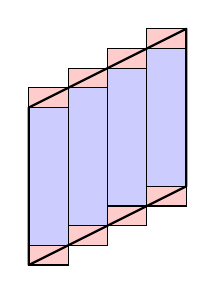
\begin{tikzpicture}[x=0.5cm, y=0.5cm]
    \draw[fill=red!20,draw=black] (0,0) -- (1,0) -- (1,0.5) -- (2,0.5) -- (2,1) -- (3,1) -- (3,1.5) -- (4,1.5) -- (4,6) 
    -- (3,6) -- (3,5.5) -- (2,5.5) -- (2,5) -- (1,5) -- (1,4.5) -- (0,4.5) -- cycle;
    \draw[fill=blue!20,draw=black] (0,0.5) -- (1,0.5) -- (1,1) -- (2,1) -- (2,1.5) -- (3,1.5) -- (3,2) -- (4,2) -- (4,5.5)
    -- (3,5.5) -- (3,5) -- (2,5) -- (2,4.5) -- (1,4.5) -- (1,4) -- (0,4) -- cycle;
    \draw (1,1) -- (1,4);
    \draw (2,1.5) -- (2,4.5);
    \draw (3,2) -- (3,5);
    \draw[thick,line join=round] (0,0) -- (4,2) -- (4,6) -- (0,4) -- cycle;
  \end{tikzpicture}}
  \caption{Approssimazione di un parallelogramma tramite polirettangoli cartesiani.}
\end{figure}

\emph{Passo 3.}
Supponiamo che sia $E=[a,b]\times[c,d]$ e $L(x,v)=(x,rx+v)$
con $r\in \RR$ fissato
(stiamo utilizzando le coordinate $(x,v)$ nel dominio di $L$
e le coordianate $(x,y)$ nel codominio).
Allora
\[
  L(E) = \{(x,y)\in \RR^2\colon x\in[a,b], rx+c \le y \le rx+d\}
\]
è un parallelogramma. 
Supponiamo per fissare le idee che sia $r\ge 0$.
Per ogni $n\in \NN$ posso affettare l'insieme
$L(E)$ con le rette verticali $x_k = a+\frac{r}{n}(b-a)$ e posso
identificare i rettangoli, per $k=1,\dots, n$:
\begin{align*}
   R_{k,n}^-
   &= \{(x,y)\in \RR^2 \colon x\in [x_{k-1},x_k), y\in[r x_k+c,r x_{k-1}+d]\},
   \\
   R_{k,n}^+
   &= \{(x,y)\in \RR^2 \colon x\in [x_{k-1},x_k), y\in[r x_{k-1}+c,r x_k+d]\}.
\end{align*}
e i polirettangoli ottenuti mettendo insieme questi rettangoli:
\begin{align*}
  P^-_n &= R_{1,n}^- \cup R_{2,n}^- \cup \dots \cup R_{n,n}^-, \\
  P^+_n & = R_{1,n}^+ \cup R_{2,n}^+ \cup \dots \cup R_{n,n}^+.
\end{align*}
Per come li abbiamo costruiti si osserva che
\[
  P^-_n \subset L(A) \subset P^+_n.
\]
Ma è facile calcolare le misure di questi polirettangoli:
\begin{align*}
  m(P^-_n) &= \sum_{k=1}^n m(R_{k,n}^-)
          = \sum_{k=1}^n(x_k-x_{k-1})\cdot (d-c-r(x_k-x_{k-1}))\\
         &= \sum_{k=1}^n \frac {b-a} n \cdot \enclose{d-c-\frac{r}{n}}
          = (b-a)\cdot \enclose{d-c-\frac{r}{n}} \\
  m(P^+) &= \sum_{k=1}^n m(R_{k,n}^+) = \dots = (b-a)\cdot \enclose{d-c+\frac{r}{n}}
\end{align*}
ma visto che per $n\to +\infty$ si ha $m(P^-_n)\to (b-a)\cdot(d-c)$
e $m(P^+_n) \to (b-a)\cdot(d-c)$ e visto che si ha
\[
  m(P^-_n)\le m_*(L(A))\le m^*(L(E)) \le m(P^+_n)
\]
otteniamo che $L(E)$ è misurabile e $m(L(E)) = (b-a)\cdot(d-c) = m(E)$.
La matrice associata ad $L$ è $M=\begin{pmatrix}1 & 0 \\ r & 1 \end{pmatrix}$
e dunque $\det M = 1$. Abbiamo quindi trovato il risultato voluto.

\emph{Passo 4.}
Sia $L$ una qualunque applicazione lineare che si ottiene come
composizione delle applicazioni considerate in precedenza: 
$L= L_n\circ \dots  \circ L_2 \circ L_1$. 
Allora per quanto già visto sappiamo
che se $E$ è un qualunque insieme Peano-Jordan misurabile risulta
\[
m(L(E)) = m\enclose{L_n(\dots(L_2(L_1(E)))\dots)}
     = \abs{\det L_n} \cdots \abs{\det L_2} \cdot \abs{\det L_1} \cdot m(E)
\]
e dunque anche $L(E)$ è Peano-Jordan misurabile e visto che
\[
 \abs{\det L} = \abs{\det L_n} \cdots \abs{\det L_1}
\]
la formula~\eqref{eq:formula_area} è verificata.

\emph{Passo 5.}
Per concludere la dimostrazione è dunque sufficiente
verificare che ogni trasformazione lineare si può scrivere come composizione delle trasformazioni già considerate.
In generale il teorema può essere formulato in dimensione qualunque (in $\RR^n$ invece che $\RR^2$) 
e la dimostrazione procede esattamente nello stesso modo considerando solo trasformazioni che coinvolgono due coordinate. 
La trasformazione che scambia due coordinate (passo 2) è rappresentata da una matrice che se moltiplicata 
a sinistra di una matrice generica $M$ ne scambia le righe, se moltiplicata a destra ne scambia le colonne. 
La trasformazione del passo 3 se applicata a sinistra somma ad una riga il multiplo di un'altra riga, 
se applicata a destra somma ad una colonna il multiplo di un'altra colonna.
Tramite il metodo di riduzione di Gauss (riduzione completa) è possibile trasformare ogni matrice 
utilizzando solamente queste trasfromazioni in modo da mantenere invariato il modulo del determinante 
e rendere la matrice diagonale. A quel punto ci siamo ricondotti al passo 1.

Nel caso planare, $n=2$, possiamo fare esplicitamente la riduzione di Gauss. 
Supponiamo che la trasformazione lineare $L$ sia associata ad una matrice generica:
\[
  M = \begin{pmatrix} a&b\\c&d\end{pmatrix}.
\]
A meno di scambiare righe e colonne possiamo supporre che sia $a\neq 0$ 
(se tutti gli elementi fossero nulli avremmo $M=0$ che è già in forma diagonale). 
Allora aggiungiamo alla seconda riga un multiplo $r$ della prima in modo da annullare il termine $b$:
\[
\begin{pmatrix} 1&0\\r&1
\end{pmatrix}\cdot
    \begin{pmatrix} a&b\\c&d
    \end{pmatrix}
  =
  \begin{pmatrix} a&b\\c+ra&d+rb
  \end{pmatrix}
\]
scegliendo $r=-\frac c a$
e ponendo $d'=d+rb$
abbiamo ottenuto la matrice:
\[
\begin{pmatrix} a&b\\0&d'
\end{pmatrix}.
\]
Ora osserviamo che
\[
      \begin{pmatrix} 0&1\\1&0
      \end{pmatrix}\cdot
      \begin{pmatrix} 1&0\\r&1
      \end{pmatrix}\cdot
      \begin{pmatrix} 0&1\\1&0
      \end{pmatrix}
      =
      \begin{pmatrix} 1&r\\0&1
      \end{pmatrix}\cdot
\]
Dunque possiamo utilizzare anche quest'ultima matrice
moltiplicandola a destra:
\[
\begin{pmatrix} a&b\\0&d'
\end{pmatrix}\cdot
  \begin{pmatrix} 1&r\\0&1
  \end{pmatrix}
  =
  \begin{pmatrix} a&ar+b\\0&d'
  \end{pmatrix}
\]
dunque scegliendo $r=-\frac b a$ si ottiene finalmente
una matrice diagonale.
\end{proof}

Il teorema precedente ci dice che la misura di un 
insieme non cambia se l'insieme viene ruotato
visto che il determinante delle isometrie è $\pm 1$. 
Ci dice anche che se dilatiamo un insieme di un fattore $\lambda$
la sua area viene moltiplicata per $\lambda^2$ 
(o $\lambda^n$ se fossimo in $\RR^n$) in quanto 
il determinante di $\lambda$ volte l'identità
è $\lambda^n$.

% section{area di un poligono}
% 
% Il teorema~\ref{th:area_lineare} ci dice che se applichiamo ad un insieme 
% $E$ una trasformazione lineare affine $L$ la cui matrice associata ha determinante 
% $1$ o $-1$, otteniamo un insieme $L(E)$ con la stessa misura.
% In particolare la misura di un insieme è invariante per isometrie:
% cioè per quelle trasformazioni la cui matrice associata è ortogonale 
% (traslazioni, rotazioni, riflessioni).
% 
% Se $E$ è un triangolo rettangolo con cateti di lunghezza $a$ e $b$ 
% a meno di rotazioni e traslazioni possiamo supporre che $E$ si ottenga 
% dividendo il rettangolo $[0,a]\times[0,b]$ lungo una diagonale. 
% Visto che le due parti in cui il rettangolo viene suddiviso sono tra 
% loro isometriche, esse devono avere ...
% 
% *** mi serve dimostrare che i poligoni sono misurabili ***

L'integrale di Riemann, che andremo a definire
nella prossima sezione, ci permetterà di osservare che ogni figura geometrica
delimitata dal grafico di una curva sufficientemente regolare risulta
essere misurabile secondo Peano-Jordan. 
Inoltre il calcolo integrale ci permetterà
di determinare l'area di tali figure in modo piuttosto semplice.

